% !TEX root = ./0.main.tex

The development of e-commerce revolutionized our shopping styles in recent years. Recommender systems play a fundamental role in e-commerce companies. 
Traditional recommendation methods mainly use collaborative filtering methods~\cite{sarwar2001item,schafer2007collaborative} to predict scores between users and items. Recently, neural networks have been widely used in e-commerce recommender systems, owing to the rapid development of deep learning. Neural recommender systems generate representations for users and items and outperform traditional recommendation methods. However, due to the large-scale e-commerce users and items, it is hard to use deep models to directly give the click-through rate (CTR) prediction between each pair of users and items. Current industrial practice is to use fast K nearest neighbors (e.g., Faiss~\cite{JDH17}) to generate the candidate items and then use a deep model (e.g., xDeepFM~\cite{lian2018xdeepfm}) to integrate the attributes of users and items to optimize the business metrics such as CTR.

% \xz{The traditional way of building up such systems mainly relies on collaborative filters, while neural-network-based models are becoming more and more popular. Modern architecture first embeds users and items, then use fast matching algorithms like fast K nearest neighbors (Faiss~\cite{JDH17}) to match these embeddings, or use more complex ways that integrate the attributes of users and items to optimize the business metrics, like xDeepFM~\cite{lian2018xdeepfm}.  } 
% Recommender systems become a fundamental part of e-commerce companies. All sorts of recommendation algorithms play an essential role in recommender systems. Traditional recommendation methods mainly use collaborative filtering to predict scores between users and items and recommend users with high-score items. Recently, neural networks have been widely used in e-commerce recommender systems, which owe to the rapid development of deep learning. Neural recommendation methods generate representations for users and items and outperform traditional recommendation algorithms.

% As we can see, the function of neural networks is to obtain the item candidates instead of giving the final recommendation list for each user.
% \xz{The problem of neural-network-based models is that they require to run. If the number of users and items scale up tremendously, for example, billions of users and items, then there's still a large gap between embeddings and final recommendations.  } 
% Excessive item pool with billions of items limits the effects of neural networks. 
Some recent works leverage graph embedding methods to obtain representations for users and items, which can be used for downstream applications. For example, PinSage~\cite{ying2018graph} builds on GraphSAGE~\cite{hamilton2017inductive} and has applied graph convolutional network based methods to production-scale data with billions of nodes and edges. GATNE~\cite{cen2019representation} considers different user behavior types and leverages a heterogeneous graph embedding method to learn representations for users and items. However, this kind of method ignores the sequential information in the user behaviors and cannot capture the correlations between adjacent user behaviors. %Also, user behaviors are updated in real time, so recommendation methods should give real-time recommendations for all users. 

Recent researches~\cite{kang2018self,chen2018sequential,lv2019sdm} formalize the recommender system as a sequential recommendation problem. With a user's behavior history, the sequential recommendation task is to predict the next item he/she might be interested in. This task reflects the real-world recommendation situation. Many recent models can give an overall embedding for each user from his/her behavior sequence. However, a unified user embedding is hard to represent multiple interests. For example, in Figure~\ref{fig:multiple_interest}, the click sequence shows three different interests of Emma. As a modern girl, Emma is interested in jewelry, handbags, and make-ups. Therefore, she may click items of the three categories during this period of time. 

% \begin{figure}
%     \centering
%     \includegraphics[width=0.45\textwidth]{figures/multiple_interests.pdf}
%     \caption{An example click sequence of a e-commerce user, Emma. The click sequence indicates that Emma has multiple interests including clothes, handbags, and makeups.}
%     \label{fig:multiple_interest}
% \end{figure}

\begin{figure*}
    \centering
    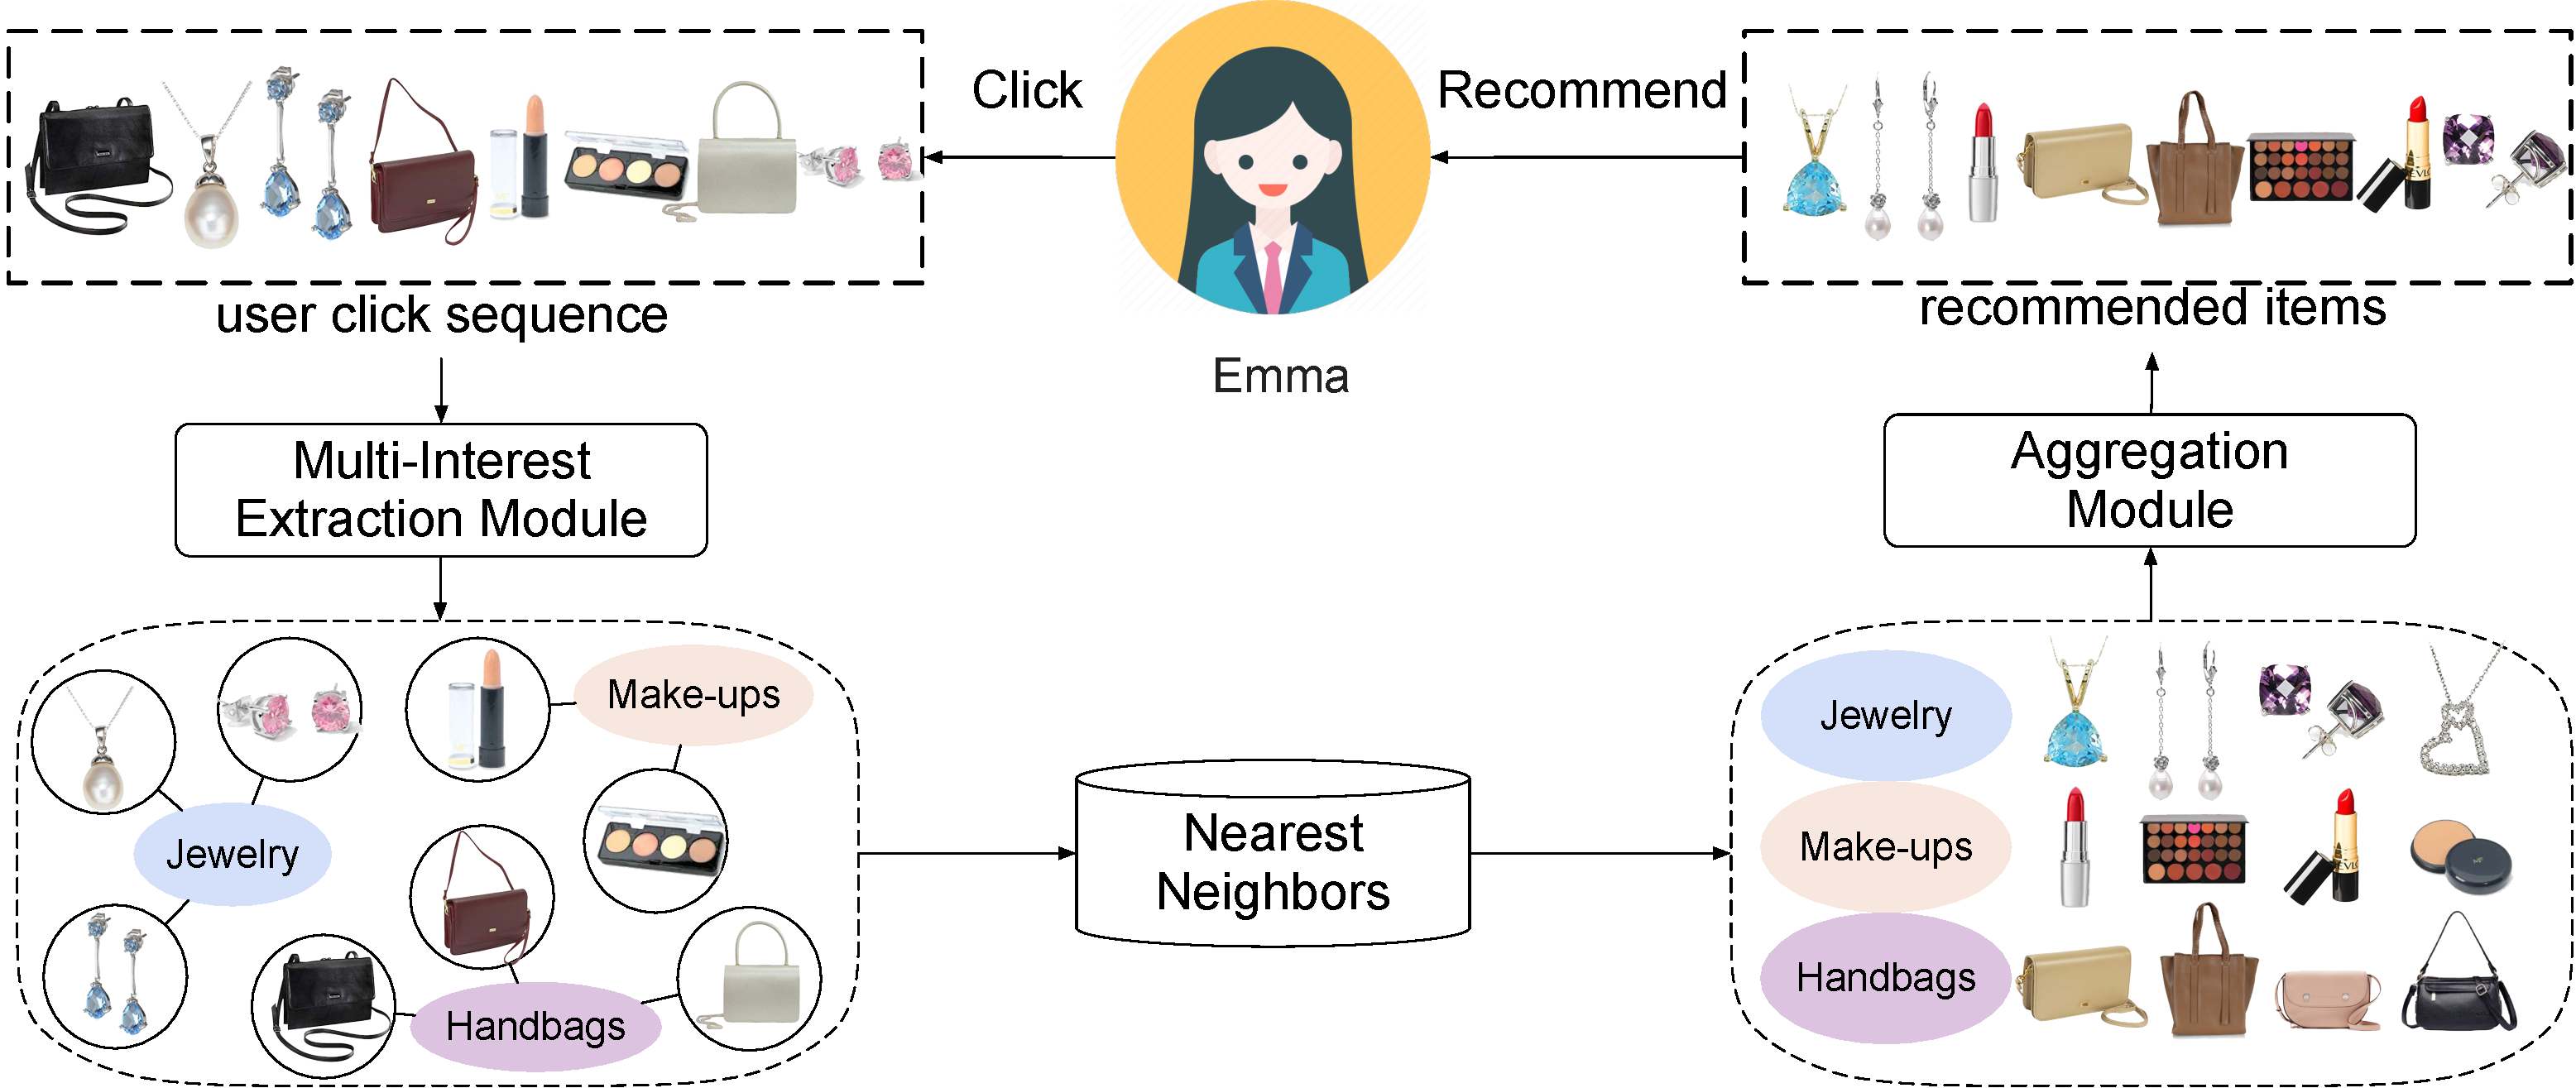
\includegraphics[width=0.8\textwidth]{figures/multi-interest-overview.pdf}
    \caption{A motivating example of our proposed framework. An e-commerce platform user, Emma, has multiple interests including jewelry, handbags, and make-ups. Our multi-interest extraction module can capture these three interests from her click sequence. Each interest retrieves items from the large-scale item pool based on the interest embedding independently. An aggregation module combines items from different interests and outputs the overall top-N recommended items for Emma. }
    \label{fig:multiple_interest}
\end{figure*}

In this paper, we propose a novel controllable multi-interest framework, called \model. Our multi-interest module can capture the multiple interests of users, which can be exploited for retrieving candidate items. Our aggregation module combines these items from different interests and outputs the overall recommendation. Figure~\ref{fig:multiple_interest} shows a motivating example of our multi-interest framework. We conduct experiments for the sequential recommendation, which is similar to our online situation. The experimental results show that our framework outperforms other state-of-the-art models. Our framework has also been successfully deployed on the Alibaba distributed cloud platform. Results on the billion-scale industrial dataset further confirm the effectiveness and efficiency of our model in practice. 

To summarize, the main contributions of this paper are:
\begin{itemize}
    \item We propose a comprehensive framework that integrates the controllability and multi-interest components in a unified recommender system. 
    \item We investigate the role of controllability on personalized systems by implementing and studying in an online recommendation scenario. 
    \item Our framework achieves state-of-the-art performance on two real-world challenging datasets for the sequential recommendation.
\end{itemize}

\iffalse
\begin{itemize}
    \item We propose a novel controllable multi-interest framework based on user sequential behaviors for sequential recommendation.
    \item The controllable module in our framework can adjust the diversity of recommended item candidates. 
    % \item We adapt the capsule network with a variation of the dynamic routing method for the multi-interest extraction. 
    \item Our framework achieves state-of-the-art results on two real-world datasets for sequential recommendation.
    % \item CapsRec has been deployed on Alibaba recommender systems and significantly improves hit rate on a billion-scale industrial dataset. 
\end{itemize} 
\fi


% \vpara{Organization}
% The rest of the paper is organized as follows. Section~\ref{sec:related} summarizes related work. Section~\ref{sec:model} formulates the sequential recommendation problem and introduces our proposed framework in detail. In Section~\ref{sec:exp}, we conduct extensive experiments and case studies. Finally, we conclude in Section~\ref{sec:conclusion}.
